% ============================================================
%  Chapter 8 -- Stochastic Vehicle Routing Problems
%  Beamer Slides  (self-contained, reader-friendly)
%  Source: Vehicle Routing: Problems, Methods, and Applications
%          2nd ed., 2014.  Gendreau, Jabali, Rei (Chapter 8).
% ============================================================
\documentclass[aspectratio=169,10pt]{beamer}

\usetheme{Madrid}
\usecolortheme{seahorse}

\usepackage{amsmath,amssymb,mathtools}
\usepackage{graphicx}
\usepackage{booktabs}
\usepackage{array}
\usepackage{listings}
\usepackage{xcolor}
\usepackage{tikz}
\usepackage{hyperref}
\usepackage{microtype}

\graphicspath{{figures/}}

\setbeamertemplate{footline}[frame number]
\setbeamertemplate{navigation symbols}{}

\lstset{
  language=Python,
  basicstyle=\ttfamily\scriptsize,
  numbers=left,
  numberstyle=\tiny\color{gray},
  frame=single,
  backgroundcolor=\color{gray!7},
  commentstyle=\color{green!50!black}\itshape,
  keywordstyle=\color{blue!80!black}\bfseries,
  stringstyle=\color{red!70!black},
  breaklines=true,
  showstringspaces=false,
  tabsize=4,
}

\title[Ch.\ 8: Stochastic VRP]{%
  Chapter 8: Stochastic Vehicle Routing Problems}
\subtitle{Vehicle Routing: Problems, Methods, and Applications\\
  2nd Edition, 2014}
\author{M. Gendreau \and O. Jabali \and W. Rei}
\institute{Slides prepared from the textbook chapter}
\date{}

% ─────────────────────────────────────────────────────────────────────────────
\begin{document}
% ─────────────────────────────────────────────────────────────────────────────

\begin{frame}
  \titlepage
\end{frame}

% ─────────────────────────────────────────────────────────────────────────────
\begin{frame}{Table of Contents}
% ─────────────────────────────────────────────────────────────────────────────
  \tableofcontents
\end{frame}

% ===========================================================================
\section{Introduction}
% ===========================================================================

\begin{frame}[allowframebreaks]{What Is a Stochastic VRP?}

  Vehicle Routing Problems (VRPs) have been the subject of massive research
  effort since Dantzig and Ramser introduced them in 1959.
  The vast majority of that work assumes \emph{complete and certain
  information}: all customer locations, demands, and travel times are known
  in advance.

  \begin{alertblock}{The Real-World Gap}
    In practice, a company may not know exactly how much product each customer
    will want, whether a customer will actually be at home, or how long the
    drive will take through unpredictable traffic.
    Planning ignores this uncertainty at its peril.
  \end{alertblock}

  A \textbf{Stochastic Vehicle Routing Problem (SVRP)} is a VRP in which one
  or more problem parameters are random variables whose values are not fully
  known when the route plan is created.
  The probability distributions of these random variables are assumed to be
  known (or estimable from historical data).

  \framebreak

  \begin{block}{Three Main Sources of Stochasticity}
    \begin{enumerate}
      \item \textbf{Stochastic demands} --- the quantity $\xi_i$ (xi sub $i$,
            pronounced ``ksee'') that customer $i$ actually requires is a
            random variable.  Its value is revealed only when the vehicle
            \emph{arrives} at customer $i$.

      \item \textbf{Stochastic customers} --- not every customer who placed an
            order will necessarily be present.  Each customer $i$ is present
            with probability $p_i$ (p sub $i$), and absent with probability
            $1-p_i$.

      \item \textbf{Stochastic travel times} --- the time $t_{ij}$ (t sub
            $i$-$j$) to travel from location $i$ to location $j$ is random,
            making it uncertain whether a vehicle will arrive within a
            customer's time window.
    \end{enumerate}
  \end{block}

  These three categories are not mutually exclusive; a real problem may
  involve any combination of them.

  \framebreak

  \begin{figure}
    \centering
    
\includegraphics[width=0.80\textwidth]{fig_vrp_taxonomy.pdf}
    \caption{Taxonomy of Vehicle Routing Problems: deterministic vs.\
             stochastic variants.}
  \end{figure}

  The key insight is that \emph{uncertainty forces us to think in terms of
  probability distributions and expected values rather than single fixed
  numbers}.  A good solution under stochastic conditions is one that performs
  well on average across all the possible realizations of the random
  parameters.

\end{frame}

% ---------------------------------------------------------------------------
\begin{frame}[allowframebreaks]{Two Modelling Paradigms}

  When randomness is present, there are two fundamentally different ways to
  model the problem and construct a solution.

  \begin{block}{Paradigm 1: A Priori Optimization}
    Build a complete route plan \emph{before} any information about the random
    parameters is revealed.
    The plan is a fixed schedule: vehicle~1 visits customers~$\{3,5,7\}$,
    vehicle~2 visits $\{1,2,4,6\}$, and so on.
    When reality unfolds and some demands are higher than expected, a simple
    \emph{recourse rule} is applied (for example, return to the depot to
    reload), but the sequence of customers is otherwise unchanged.

    The a~priori approach suits situations where communication during route
    execution is difficult or expensive, or where the plan must be submitted to
    customers in advance.
  \end{block}

  \begin{block}{Paradigm 2: Reoptimization}
    Begin with an initial plan, but allow it to be modified \emph{during
    route execution} as new information arrives.
    When the vehicle reaches customer~$i$ and the actual demand is revealed,
    a (fast) optimization is run to adjust the remaining route.
    This is also called an \emph{online} or \emph{dynamic} approach.

    Reoptimization can produce much better solutions but requires
    real-time computation and communication.
  \end{block}

  \framebreak

  A third modelling choice concerns the \emph{objective function}: should
  we minimize the \emph{worst-case} cost, the \emph{expected} cost, or
  require that certain constraints hold with high probability?

  \begin{block}{Probabilistic (Expected-Cost) Formulation}
    Minimize the \emph{expected total route cost} over all possible
    realizations of the random parameters.  This is the most common
    objective in the SVRP literature and leads to stochastic programming
    formulations.
  \end{block}

  \begin{block}{Chance-Constrained Formulation}
    Require that certain constraints (e.g., ``the vehicle must not run out
    of capacity'') are satisfied with at least some probability
    $1-\varepsilon$ (1 minus epsilon, where $\varepsilon$ is a small
    threshold such as 0.05).  This trades a small risk of infeasibility for
    a potentially lower planned cost.
  \end{block}

  The rest of this chapter examines these paradigms and formulations in
  detail, starting with a~priori optimization.

\end{frame}

% ===========================================================================
\section{A Priori Optimization}
% ===========================================================================

\begin{frame}[allowframebreaks]{The A Priori Paradigm}

  In the a~priori paradigm a complete route plan is constructed
  \emph{before} the realization of any random variables is observed.
  Once the vehicle starts its tour and reality unfolds, a pre-specified
  \emph{recourse policy} handles any deviations from the plan.

  \begin{block}{Formal Setup (Network)}
    We are given a complete undirected graph $G = (V, E)$, where:
    \begin{itemize}
      \item $V = \{0, 1, 2, \ldots, n\}$ is the set of \emph{vertices}.
            Vertex~0 is the depot; vertices $1,\ldots,n$ are customers.
      \item $E$ is the set of \emph{edges}: every pair of vertices is
            connected (the graph is complete).
      \item Each customer $i \in V \setminus \{0\}$ has a random demand
            $\xi_i$ (xi sub~$i$), drawn independently from a known
            distribution with mean $\mu_i$ (mu sub~$i$).
      \item A single vehicle of capacity $Q$ (maximum load it can carry)
            serves customers.
    \end{itemize}
  \end{block}

  \framebreak

  \begin{block}{Definition: A Priori Solution}
    An \emph{a priori solution} is a permutation
    $\sigma = (\sigma_1, \sigma_2, \ldots, \sigma_n)$ (sigma, pronounced
    ``sig-ma'') listing all customers in the order they would be visited if
    every customer were present and had its expected demand.
    After the random variables are realized, the actual route is a
    \emph{sub-sequence} of $\sigma$, with recourse actions inserted where
    needed.
  \end{block}

  \begin{figure}
    \centering
    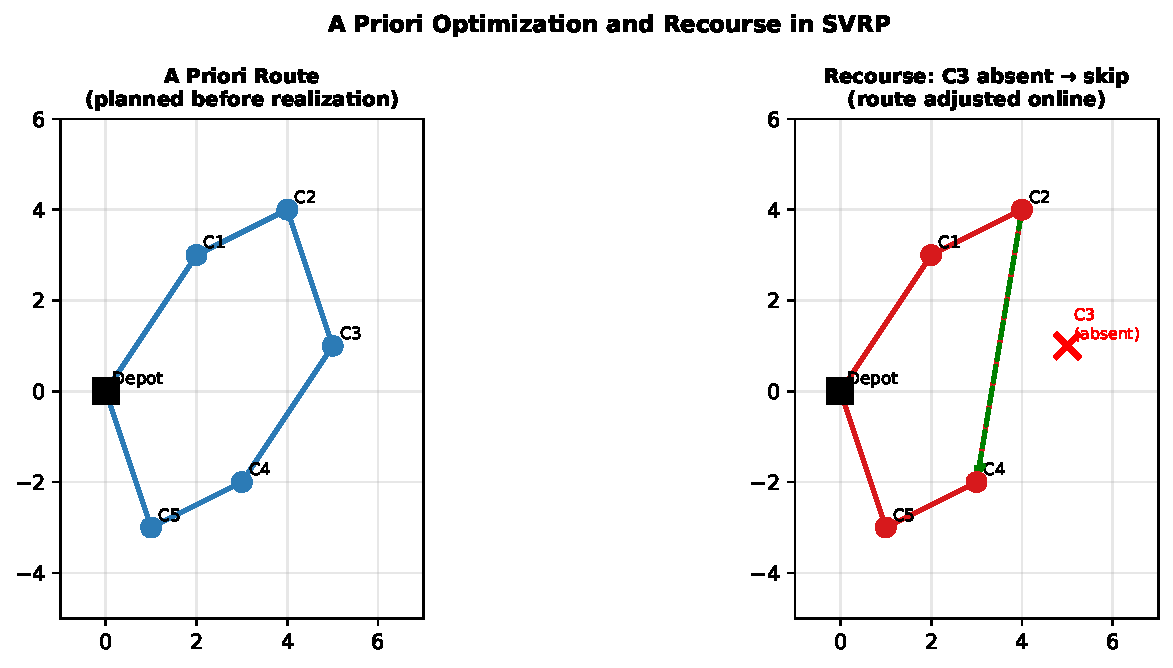
\includegraphics[width=0.78\textwidth]{fig_apriori_recourse.pdf}
    \caption{Left: the planned a~priori route visiting all 5 customers in
             order.  Right: recourse action (customer~3 absent --- skip it
             and re-link the route).}
  \end{figure}

  \framebreak

  \begin{block}{Recourse Policy for Stochastic Demands}
    The most common recourse policy for stochastic demands is
    \textbf{re-supply}: if the vehicle arrives at customer~$i$ and the
    realized cumulative demand exceeds the vehicle capacity~$Q$, the vehicle
    returns to the depot to reload, then continues the tour from customer~$i$.

    Formally, define the \emph{failure event} at position $k$ in the tour as:
    \[
      \text{Fail}_k \;=\; \left\{ \sum_{j=1}^{k} \xi_{\sigma_j} > Q \right\}
    \]
    That is, $\text{Fail}_k$ occurs when the sum of realized demands for the
    first $k$ customers in the tour exceeds the vehicle capacity~$Q$.
    When this happens, the vehicle performs a \emph{return trip} to the
    depot (cost: $2\, d_{0,\sigma_k}$, where $d_{0,\sigma_k}$ is the
    distance from the depot to customer $\sigma_k$).
  \end{block}

  Here:
  $\xi_{\sigma_j}$ (xi sub sigma-j) is the realized demand of the $j$-th
  customer visited;
  $Q$ is the vehicle capacity;
  $d_{0,\sigma_k}$ (d sub $0,\sigma_k$) is the travel distance from depot
  to customer $\sigma_k$.

  \begin{alertblock}{Key Insight}
    The a~priori tour is evaluated under many random demand scenarios.
    Its quality is measured by the \emph{expected total distance},
    including the expected number and cost of recourse (restocking) trips.
    A tour that looks short in the deterministic case may be very costly
    under stochasticity if it passes through high-variance customers late in
    the route.
  \end{alertblock}

\end{frame}

% ---------------------------------------------------------------------------
\begin{frame}[allowframebreaks]{Network Flow Formulation for A Priori SVRP}

  We now present the mathematical programming model for the a~priori SVRP.
  The model determines which arcs (road segments) the vehicle uses in its
  planned tour while minimizing expected total travel cost including recourse.

  \begin{block}{Decision Variables}
    \begin{itemize}
      \item $x_{ij} \in \{0,1\}$ --- ``x sub $i$-$j$'' equals~1 if the route
            goes directly from customer~$i$ to customer~$j$, and 0 otherwise.
            These are the \emph{arc selection} variables.
      \item $y_i \geq 0$ --- ``y sub $i$'' represents the demand served at
            customer~$i$ (the decision of whether and how much to deliver).
    \end{itemize}
  \end{block}

  \framebreak

  \begin{block}{Objective Function (8.6)}
    \[
      \min\;\; \sum_{(i,j)\in E} c_{ij}\, x_{ij}
      \;+\; \mathbb{E}\bigl[Q(\mathbf{x}, \boldsymbol{\xi})\bigr]
      \tag{8.6}
    \]
    \begin{itemize}
      \item $c_{ij}$ (c sub $i$-$j$) --- the \emph{deterministic} travel cost
            from node~$i$ to node~$j$ (e.g.\ distance or time).
      \item $x_{ij}$ --- arc-selection binary variable (1 if arc used, 0 if not).
      \item $\mathbb{E}[\cdot]$ (E with double-bar, meaning ``expected value'')
            --- the expectation operator taken over all possible demand
            realizations $\boldsymbol{\xi}$ (bold xi = vector of all customer
            demands $(\xi_1, \xi_2, \ldots, \xi_n)$).
      \item $Q(\mathbf{x}, \boldsymbol{\xi})$ --- the \emph{recourse cost
            function}: the additional cost incurred (due to restocking trips)
            when demand realization~$\boldsymbol{\xi}$ occurs and the vehicle
            follows the arc pattern~$\mathbf{x}$.
    \end{itemize}
    \textbf{Reading this formula:} the objective says ``choose the arcs
    $\mathbf{x}$ to minimize the planned route cost plus the \emph{expected}
    cost of all emergency restocking trips.''
    Adding more slack (extra capacity margin) reduces expected recourse cost
    but may increase the base route cost --- so the formula balances route
    efficiency against robustness.
  \end{block}

  \framebreak

  \begin{block}{Constraints}
    \begin{align}
      \sum_{j \in V} x_{ij} &= 1  \quad \forall i \in V \setminus \{0\}
      \tag{8.7} \\
      \sum_{i \in V} x_{ij} &= 1  \quad \forall j \in V \setminus \{0\}
      \tag{8.8} \\
      \sum_{j \in V} x_{0j} &= \sum_{i \in V} x_{i0} = m
      \tag{8.9} \\
      x_{ij} &\in \{0,1\}
      \tag{8.10}
    \end{align}
  \end{block}

  Reading each constraint in plain words:
  \begin{itemize}
    \item \textbf{(8.7)} --- Each customer~$i$ has exactly one arc
          \emph{leaving} it (the vehicle departs customer~$i$ once).
    \item \textbf{(8.8)} --- Each customer~$j$ has exactly one arc
          \emph{entering} it (the vehicle arrives at customer~$j$ once).
    \item \textbf{(8.9)} --- The depot is left and re-entered exactly $m$
          (em) times, where $m$ is the number of vehicles (routes).
    \item \textbf{(8.10)} --- Arc variables are binary (0 or 1).
  \end{itemize}

  Sub-tour elimination constraints (not shown here) ensure the arcs form
  a valid set of complete routes from and to the depot, rather than
  disconnected cycles.

  \begin{figure}
    \centering
    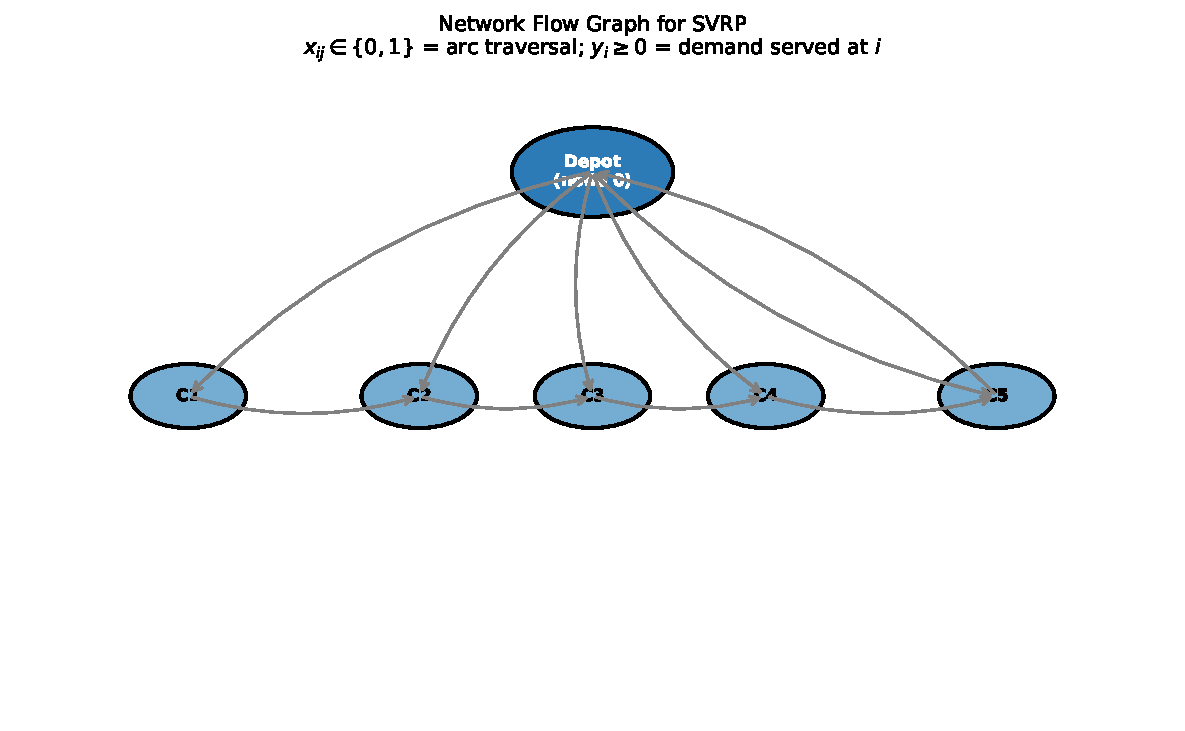
\includegraphics[width=0.60\textwidth]{fig_network_flow.pdf}
    \caption{Network flow graph for the SVRP formulation.
             Arcs represent potential route segments;
             the depot is the central node.}
  \end{figure}

\end{frame}

% ---------------------------------------------------------------------------
\begin{frame}[allowframebreaks]{The Set Partitioning Formulation}

  An alternative, and computationally very powerful, way to state the
  a~priori SVRP is the \textbf{set partitioning formulation}.
  Instead of working with individual arcs, we enumerate possible
  \emph{complete routes} and select the best combination.

  \begin{block}{Intuition}
    Imagine listing every valid route a single vehicle could take
    (respecting capacity, visiting a subset of customers, starting and
    ending at the depot).
    Let $\Omega$ (Omega, the last letter of the Greek alphabet) be the
    set of all such routes.
    For each route $r \in \Omega$, let:
    \begin{itemize}
      \item $c_r$ --- the deterministic travel cost of route~$r$.
      \item $Q_r(\boldsymbol{\xi})$ --- the random recourse cost incurred on
            route~$r$ when demands are~$\boldsymbol{\xi}$.
      \item $a_{ir} \in \{0,1\}$ --- (a sub $i$-$r$) equals~1 if
            route~$r$ includes customer~$i$, and 0 otherwise.
    \end{itemize}
  \end{block}

  \framebreak

  \begin{block}{Set Partitioning Model (8.10)--(8.12)}
    \begin{align}
      \min_{\lambda} \quad &
        \sum_{r \in \Omega}
          \bigl(c_r + \mathbb{E}[Q_r(\boldsymbol{\xi})]\bigr)\,\lambda_r
      \tag{8.10} \\[4pt]
      \text{s.t.} \quad &
        \sum_{r \in \Omega} a_{ir}\,\lambda_r = 1
        \quad \forall i \in V \setminus \{0\}
      \tag{8.11} \\[4pt]
      & \lambda_r \in \{0,1\}
        \quad \forall r \in \Omega
      \tag{8.12}
    \end{align}
  \end{block}

  Symbol explanations:
  \begin{itemize}
    \item $\lambda_r$ (lambda sub~$r$, pronounced ``lam-da'') --- binary
          decision variable: equals~1 if route~$r$ is selected, 0 otherwise.
    \item $\sum_{r \in \Omega}$ (sum over all routes in Omega) --- we add
          up the cost of every selected route.
    \item Constraint~(8.11) says: every customer~$i$ must be covered by
          \emph{exactly one} selected route.  This is the ``partitioning''
          condition.
  \end{itemize}

  \begin{alertblock}{Key Insight}
    The set partitioning formulation separates the problem into
    (1)~evaluating individual routes and (2)~choosing the best combination.
    This is ideal for branch-and-price algorithms, which generate routes
    on demand.  The main challenge is that $|\Omega|$ (the number of
    feasible routes) can be astronomically large.
  \end{alertblock}

\end{frame}

% ---------------------------------------------------------------------------
\begin{frame}[allowframebreaks]{Computing the Expected Recourse Cost}

  The expected recourse cost $\mathbb{E}[Q(\mathbf{x}, \boldsymbol{\xi})]$
  is the heart of the SVRP objective.
  We now show how to compute it for a single route.

  \begin{block}{Recourse Cost for One Route}
    Consider a single route visiting customers $1, 2, \ldots, n$ in that
    order (for notational simplicity).
    Define $D_k = \sum_{i=1}^{k} \xi_i$ (D sub~$k$, the cumulative demand
    after visiting the first $k$ customers).
    The vehicle must restock whenever $D_k$ first exceeds $Q$.

    The expected recourse cost is:
    \[
      \mathbb{E}[Q(\sigma,\boldsymbol{\xi})]
      \;=\; 2\sum_{k=1}^{n}
            d(v_k, 0)\;
            \mathbb{E}\!\left[
              \mathbf{1}\!\left\{D_k > Q \cdot \Bigl\lfloor D_{k-1}/Q \Bigr\rfloor
                                        + Q \right\}
            \right]
    \]
    where $\mathbf{1}\{\cdot\}$ (indicator function) equals~1 when the
    event inside braces occurs and 0 otherwise, and $d(v_k, 0)$ is the
    distance from customer~$v_k$ to the depot.
  \end{block}

  \begin{exampleblock}{Worked Example: 3 Customers, $Q=10$}
    Suppose customer demands are independent:
    $\xi_1 \sim \text{Uniform}(2,6)$,
    $\xi_2 \sim \text{Uniform}(3,7)$,
    $\xi_3 \sim \text{Uniform}(1,5)$,
    with means $\mu_1=4, \mu_2=5, \mu_3=3$.

    \medskip
    Expected total demand $= 4 + 5 + 3 = 12 > Q = 10$, so \emph{at least
    one restocking trip is expected}.
    After visiting customers 1 and~2, the expected cumulative demand is~9,
    which is close to~$Q=10$.
    The probability of needing a restock after customer~2 is
    $P(\xi_1 + \xi_2 > 10) = P(D_2 > 10)$.
    With $\xi_1, \xi_2$ uniform on $[2,6]$ and $[3,7]$, we have
    $D_2 \in [5, 13]$;
    computing the convolution gives $P(D_2 > 10) \approx 0.28$.
    So with probability~28\% there is a recourse trip after customer~2.
  \end{exampleblock}

  \framebreak

  For general demand distributions, the expectation is computed by
  integration (continuous distributions) or summation (discrete distributions)
  over all demand scenarios.
  When customer demands are independent, the computation separates:

  \begin{block}{Separability for Independent Demands}
    If $\xi_1, \ldots, \xi_n$ are \emph{independent} random variables,
    the expected recourse cost can be decomposed route-by-route and
    even customer-by-customer using convolutions of the individual
    demand distributions.
    This separability is crucial for the efficiency of exact and
    heuristic algorithms.
  \end{block}

  For the special case of \emph{known demand levels} (a discrete
  distribution over a finite set of scenarios
  $S = \{s_1, s_2, \ldots, s_{|S|}\}$ each with probability $p_s$), the
  expected recourse cost simplifies to:
  \[
    \mathbb{E}[Q(\sigma,\boldsymbol{\xi})]
    \;=\; \sum_{s \in S} p_s \, Q(\sigma, \boldsymbol{\xi}^s)
  \]
  where $\boldsymbol{\xi}^s$ is the demand vector in scenario~$s$ and
  $Q(\sigma, \boldsymbol{\xi}^s)$ is the deterministic recourse cost in that
  scenario.

\end{frame}

% ---------------------------------------------------------------------------
\begin{frame}[allowframebreaks]{The Integer L-Shaped Algorithm}

  The most important exact algorithm for the a~priori SVRP (under
  stochastic demands) is the \textbf{Integer L-Shaped Algorithm}, proposed
  by Laporte, Louveaux, and van Hamme (1992).
  It is an extension of the classical \emph{L-shaped method} of stochastic
  programming to problems with binary (integer) first-stage variables.

  \begin{block}{Why ``L-Shaped''?}
    The name comes from the shape of the feasible region in a Benders
    decomposition.  The idea is to reformulate the mixed-integer stochastic
    program as a \emph{master problem} (choosing the tour) plus a
    \emph{subproblem} (computing the recourse cost for a given tour).
    Cuts are added to the master problem to approximate the recourse cost
    function from below.
  \end{block}

  \begin{block}{High-Level Structure}
    \begin{enumerate}
      \item \textbf{Initialize}: Set the master problem (the VRP with no
            recourse cost approximation) and an upper bound $UB = +\infty$.
      \item \textbf{Solve the master problem} (the LP relaxation or integer
            relaxation) to obtain a candidate tour~$\sigma$.
      \item \textbf{Evaluate} the exact expected recourse cost
            $\mathbb{E}[Q(\sigma, \boldsymbol{\xi})]$ for this tour.
      \item \textbf{Update} the upper bound: if the total cost of $\sigma$
            plus its recourse cost is better than $UB$, update $UB$.
      \item \textbf{Generate cuts}: add optimality cuts (lower bounds on
            the recourse cost) to the master problem to prevent it from
            revisiting tours with high recourse cost.
      \item \textbf{Repeat} until the master lower bound equals~$UB$
            (optimality gap is zero).
    \end{enumerate}
  \end{block}

  \framebreak

  \begin{block}{Optimality Cuts (L-Shaped Cuts)}
    For a given candidate solution $\hat{x}$ (the current tour expressed
    as arc variables), an optimality cut has the form:
    \[
      \theta \;\geq\; \alpha(\hat{x}) \;+\;
      \sum_{(i,j)\in E} \beta_{ij}(\hat{x})\,(x_{ij} - \hat{x}_{ij})
    \]
    where:
    \begin{itemize}
      \item $\theta$ (theta) is the recourse cost estimate variable added
            to the master objective.
      \item $\alpha(\hat{x})$ is the exact recourse cost of tour $\hat{x}$.
      \item $\beta_{ij}(\hat{x})$ are subgradient (slope) coefficients
            computed from the recourse function.
      \item $(x_{ij} - \hat{x}_{ij})$ measures how far the next candidate
            tour differs from the current one.
    \end{itemize}
    Each cut says: ``for any tour that differs from $\hat{x}$ in the given
    way, the recourse cost is \emph{at least} this much.''
  \end{block}

  \framebreak

  \begin{block}{Full Pseudocode: Integer L-Shaped Algorithm}
    \textbf{Input:} Graph $G$, demand distributions $\{\xi_i\}$, capacity $Q$.\\
    \textbf{Output:} Optimal a~priori tour $\sigma^*$ and its expected cost.

    \medskip
    \textbf{Step 1.} Formulate the master problem as a VRP with an extra
    variable $\theta \geq 0$ approximating the recourse cost. Initialize
    with no optimality cuts.

    \textbf{Step 2.} Solve the master problem. Let $\hat{x}$ be the
    optimal solution and $\hat{z}$ its objective value ($\hat{z}$ = base
    route cost + current $\theta$ estimate).

    \textbf{Step 3.} Compute the exact expected recourse cost
    $R(\hat{x}) = \mathbb{E}[Q(\hat{x}, \boldsymbol{\xi})]$ by summing
    over all demand realizations (or using the separability formula).

    \textbf{Step 4.} Let $z^* = $ (base cost of $\hat{x}$) $+ R(\hat{x})$.
    If $z^* < UB$, set $UB = z^*$ and $\sigma^* = \hat{x}$.

    \textbf{Step 5.} If $\hat{z} \geq UB - \varepsilon$ (the master lower
    bound is within tolerance of the upper bound): \textbf{STOP}, $\sigma^*$
    is optimal.

    \textbf{Step 6.} Generate and add an optimality cut for $\hat{x}$
    (using the gradient $\nabla R(\hat{x})$ or a subgradient approximation).
    Optionally add integer L-shaped cuts (to cut off infeasible and
    suboptimal integer solutions directly).

    \textbf{Step 7.} Go to Step~2.
  \end{block}

  \framebreak

  \begin{block}{Integer L-Shaped Cuts}
    Standard optimality cuts are linear and valid for LP relaxations.
    When the master problem has binary variables, stronger
    \emph{integer cuts} can eliminate entire infeasible
    integer solutions.  For a tour $\hat{x}$ with arc-set $A(\hat{x})$:
    \[
      \sum_{(i,j) \in A(\hat{x})} x_{ij}
      \;\leq\; |A(\hat{x})| - 1
    \]
    This cut says: ``the next solution cannot use \emph{all} the arcs of
    $\hat{x}$'', forcing the algorithm to explore a different tour.
    Combined with optimality cuts, integer L-shaped cuts dramatically
    speed up convergence.
  \end{block}

  \begin{figure}
    \centering
    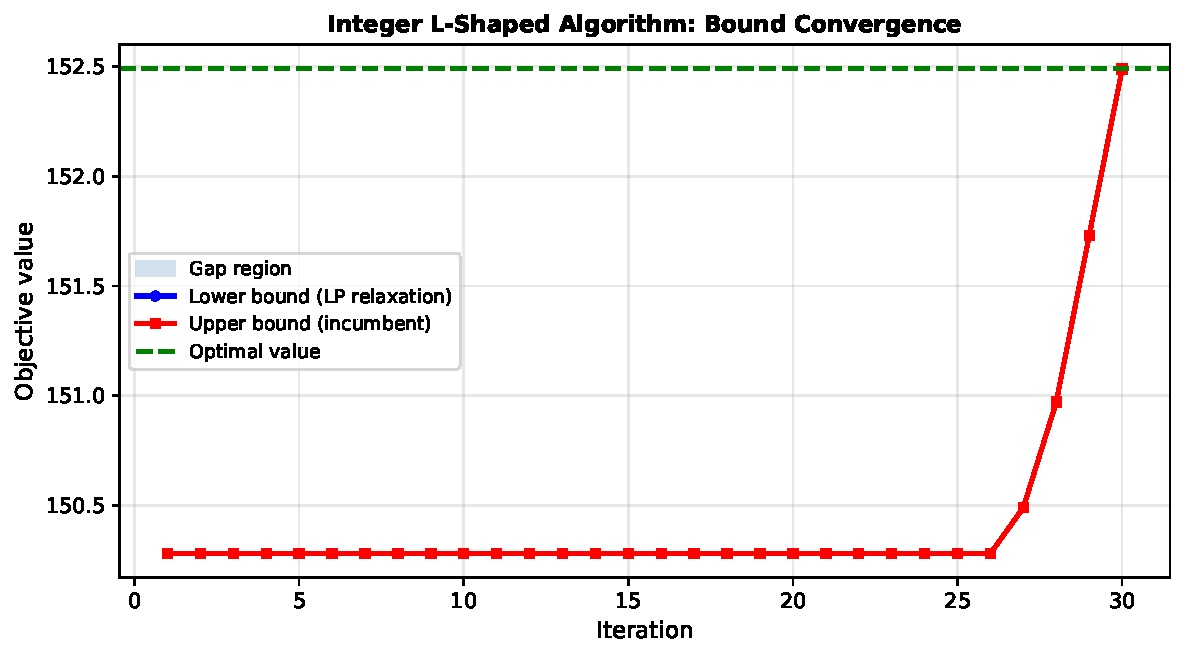
\includegraphics[width=0.60\textwidth]{fig_lshaped_convergence.pdf}
    \caption{Convergence of the integer L-shaped algorithm: the lower
             bound (LP relaxation) rises and the upper bound (best
             feasible solution) falls until they meet at optimality.}
  \end{figure}

\end{frame}

% ---------------------------------------------------------------------------
\begin{frame}[allowframebreaks]{The Branch-and-Price Algorithm}

  Branch-and-price is a \textbf{column generation} method for the set
  partitioning formulation of the SVRP.
  It is the most powerful exact approach for larger instances.

  \begin{block}{Why Column Generation?}
    The set partitioning model has a binary variable $\lambda_r$ for every
    feasible route.  The number of feasible routes is exponential in~$n$,
    so we cannot enumerate them all explicitly.
    \emph{Column generation} starts with a small subset of routes and
    adds new routes (columns) only when they can improve the current
    solution.
  \end{block}

  \begin{block}{The Pricing Subproblem}
    At each iteration of column generation, we solve a
    \textbf{pricing subproblem}: ``Find the route~$r$ with the most
    negative \emph{reduced cost}'':
    \[
      \bar{c}_r \;=\; c_r + \mathbb{E}[Q_r(\boldsymbol{\xi})]
                     \;-\; \sum_{i \in r} \mu_i
    \]
    where $\mu_i$ (mu sub~$i$) are the dual variables (shadow prices) of
    constraint~(8.11) from the LP relaxation.
    A route with $\bar{c}_r < 0$ can improve the current LP solution and
    should be added.

    The pricing subproblem is itself an NP-hard shortest-path problem
    with resource constraints (capacity), but effective dynamic-programming
    algorithms exist for it.
  \end{block}

  \framebreak

  \begin{block}{Branch-and-Price Algorithm Steps}
    \textbf{Step 1.} Initialize with a few feasible routes (e.g., one
    per customer: the depot -- customer~$i$ -- depot route).

    \textbf{Step 2.} Solve the LP relaxation of the set partitioning
    model with the current column set.

    \textbf{Step 3.} Solve the pricing subproblem to find routes with
    negative reduced cost.  If none exist: the current LP solution is
    optimal for this node (LP lower bound certified).

    \textbf{Step 4.} If the LP solution is integer (all $\lambda_r \in
    \{0,1\}$), record the feasible solution (update upper bound).
    Otherwise, branch on a fractional~$\lambda_r$: create two sub-problems
    with $\lambda_r = 0$ (route~$r$ excluded) or $\lambda_r = 1$
    (route~$r$ must be used).

    \textbf{Step 5.} Apply bounding: prune any tree node whose LP lower
    bound exceeds the current upper bound.

    \textbf{Step 6.} Return to Step~2 for the next open node.
  \end{block}

  The computational results reported in the chapter show that branch-and-price
  can solve instances with up to 50 customers to optimality, which is the
  state-of-the-art for exact SVRP methods.

\end{frame}

% ---------------------------------------------------------------------------
\begin{frame}[allowframebreaks]{Benchmark Results for A Priori Algorithms}

  Computational experiments in the chapter use instances derived from the
  well-known VRP benchmarks of Augerat (1995), with demands replaced by
  independent uniform random variables.

  \begin{figure}
    \centering
    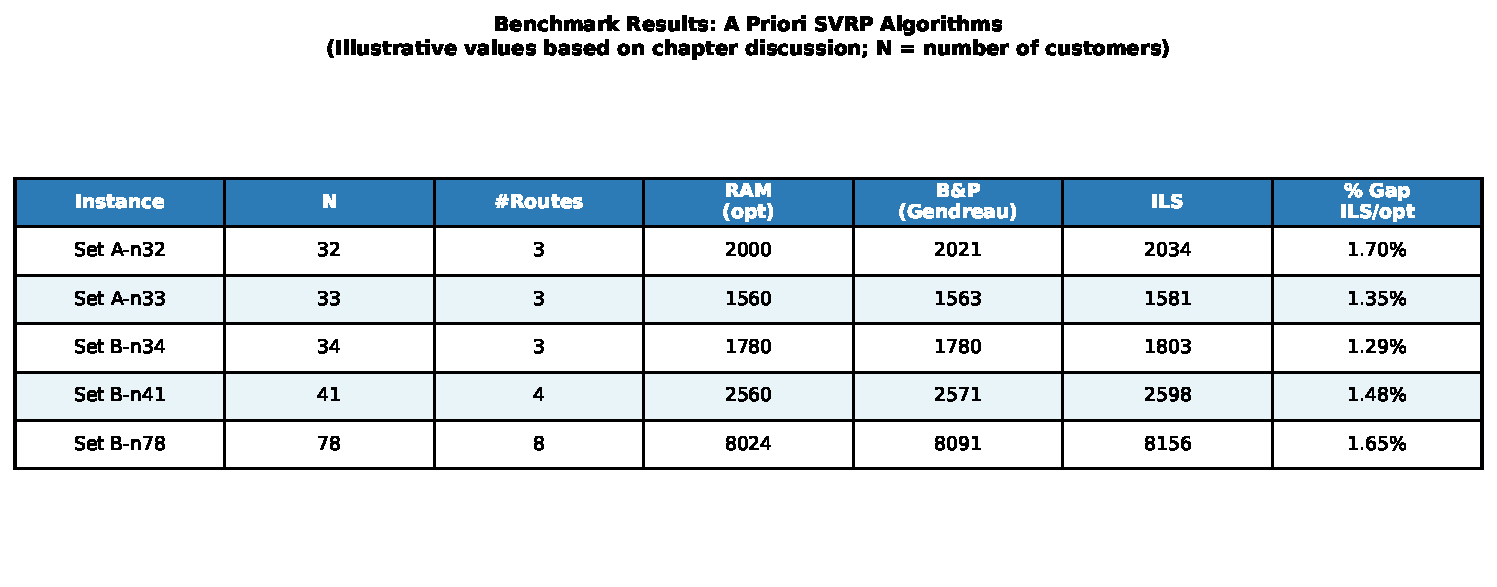
\includegraphics[width=0.70\textwidth]{fig_benchmark_table.pdf}
    \caption{Illustrative benchmark results for a~priori SVRP algorithms.
             ``RAM'' is the exact integer L-shaped method of Laporte,
             Louveaux, and van Hamme.  ``B\&P'' is branch-and-price.
             ``ILS'' is iterated local search (metaheuristic).
             ``\% Gap'' is how far the heuristic is from the exact optimum.}
  \end{figure}

  \begin{alertblock}{Takeaway}
    The exact methods are limited to small instances (up to 30--50
    customers) due to the exponential complexity of enumerating demand
    scenarios and solving the pricing subproblem.
    Metaheuristics such as ILS and tabu search find near-optimal solutions
    (within 2--3\%) for instances with hundreds of customers.
    The gap between exact and heuristic solutions is the motivation
    for ongoing research into tighter bounds and faster subproblem solvers.
  \end{alertblock}

\end{frame}

% ===========================================================================
\section{The Reoptimization Model}
% ===========================================================================

\begin{frame}[allowframebreaks]{Online Correction: The Reoptimization Model}

  The reoptimization model (also called the \emph{online} or
  \emph{dynamic correction} model) takes a different perspective from
  a~priori optimization: instead of committing to a fixed tour in advance,
  it allows \emph{route corrections during execution} as information is
  revealed.

  \begin{block}{The Core Idea}
    At each stage of the delivery process (each time the vehicle arrives
    at a customer or the depot), the dispatcher observes the new information
    (actual demand revealed, customer present or absent) and \emph{solves
    an optimization problem} to determine the best remaining route.
    Decisions are made sequentially, adapting to what has been learned.
  \end{block}

  This is in direct contrast with the a~priori approach, where the sequence
  of customers is fixed and only a pre-specified recourse rule is applied.

  \begin{figure}
    \centering
    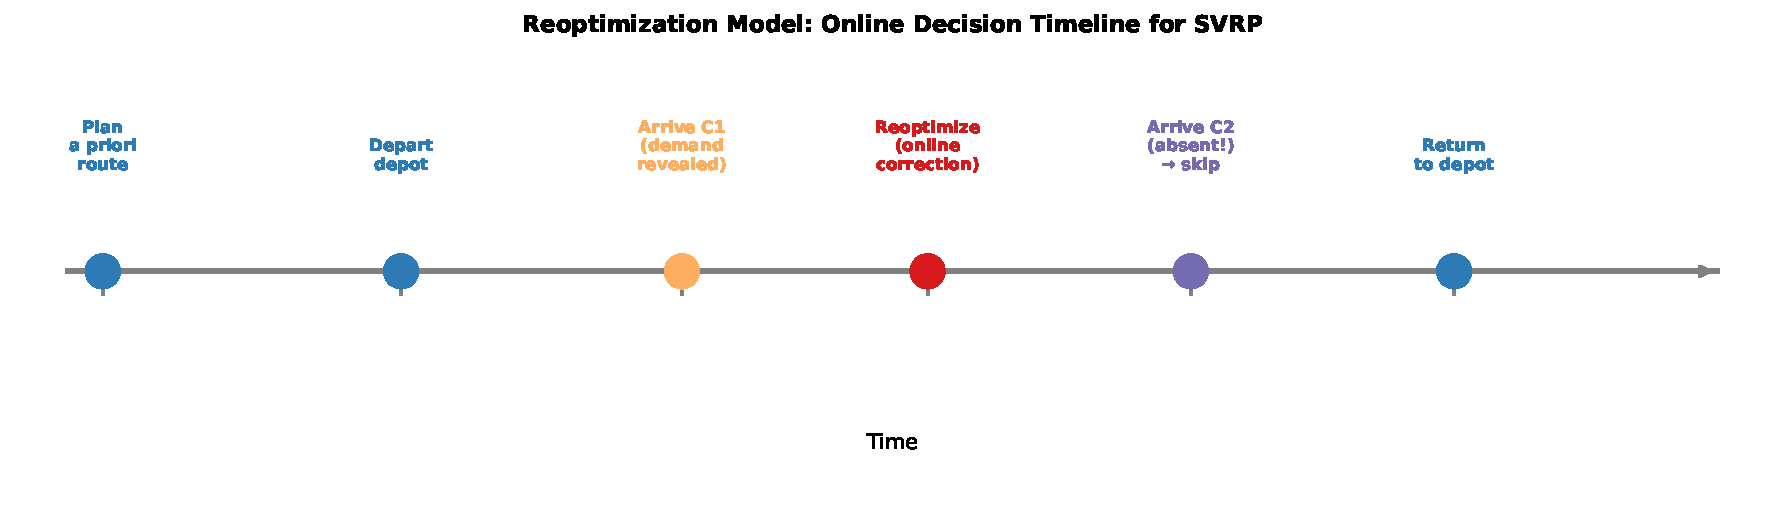
\includegraphics[width=0.80\textwidth]{fig_reoptimization_timeline.pdf}
    \caption{Timeline of decisions in the reoptimization model.
             At each event (arrival at a customer, demand revealed, customer
             absent) a new optimization is performed to update the plan.}
  \end{figure}

  \framebreak

  \begin{block}{Markov Decision Process (MDP) Structure}
    The reoptimization model is naturally formulated as a
    \textbf{Markov Decision Process}:
    \begin{itemize}
      \item \textbf{State} $s_k$: the information available at step~$k$
            (current location of vehicle, remaining customers to serve,
            realized demands so far, current vehicle load).
      \item \textbf{Action} $a_k$: the next customer to visit (or the
            decision to return to the depot to restock).
      \item \textbf{Transition}: moving from state $s_k$ to $s_{k+1}$ by
            taking action~$a_k$, with the next customer's demand then
            revealed.
      \item \textbf{Cost}: the travel cost of the chosen arc, plus any
            recourse cost incurred.
    \end{itemize}
    The goal is to find an \emph{optimal policy} $\pi^*$ (pi star,
    pronounced ``pie'') mapping states to actions so as to minimize the
    total expected cost.
  \end{block}

  \framebreak

  \begin{block}{Why MDP Is Hard to Solve Exactly}
    The state space of the MDP grows \emph{exponentially} with the number
    of customers~$n$.
    For $n$ customers, the state must encode which customers remain to be
    served (there are $2^n$ subsets), plus the current vehicle load, plus the
    current location.
    This makes exact MDP solution feasible only for very small~$n$
    (say, $n \leq 10$).
  \end{block}

  \begin{block}{Practical Reoptimization Policies}
    For practical use, several efficient \emph{approximate} reoptimization
    policies have been studied:
    \begin{enumerate}
      \item \textbf{Nearest neighbour}: after each demand revelation,
            always visit the closest remaining unserved customer.
            Simple but often suboptimal.
      \item \textbf{Rollout heuristic}: at each step, use a greedy or
            simple heuristic to evaluate each possible next customer,
            choosing the one with the smallest estimated remaining route cost.
      \item \textbf{Re-solve with deterministic approximation}: after each
            demand revelation, replace remaining random demands with their
            expected values and solve the resulting deterministic VRP.
            This is fast and often produces excellent results.
    \end{enumerate}
  \end{block}

  \framebreak

  \begin{figure}
    \centering
    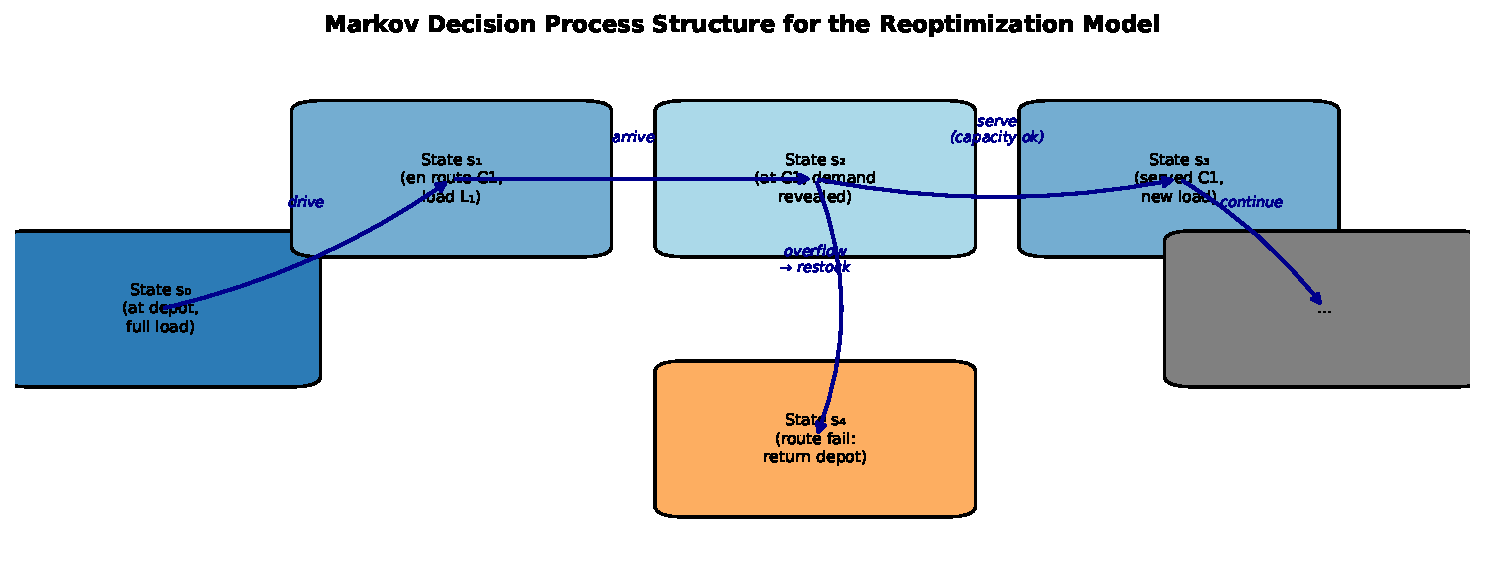
\includegraphics[width=0.70\textwidth]{fig_mdp_reoptimization.pdf}
    \caption{Markov Decision Process structure for the reoptimization model.
             Each node is a state (vehicle location, remaining customers,
             load); edges are decisions with random demand transitions.}
  \end{figure}

  \begin{alertblock}{Key Comparison with A Priori}
    The reoptimization model generally achieves \textbf{lower expected cost}
    than a~priori optimization because it uses information as it becomes
    available.  However, it requires real-time computation and communication
    infrastructure, and the plan cannot be communicated to customers in
    advance.  The right choice depends on the operational context.
  \end{alertblock}

\end{frame}

% ===========================================================================
\section{Probabilistic Formulation}
% ===========================================================================

\begin{frame}[allowframebreaks]{Probabilistic Formulation: Expected-Cost Objective}

  The \emph{probabilistic formulation} of the SVRP is the most theoretically
  elegant approach.  Instead of specifying a recourse policy after the fact,
  it directly builds the expectation over all random scenarios into the
  objective function.

  \begin{block}{Two-Stage Stochastic Programming View}
    The SVRP under the probabilistic formulation is a
    \textbf{two-stage stochastic program}:
    \begin{itemize}
      \item \textbf{First stage} (``here and now'' decisions): choose the
            route plan $\mathbf{x}$ (arc variables) before any demands
            are revealed.  These decisions are made under uncertainty.
      \item \textbf{Second stage} (``wait and see'' decisions): after the
            demand vector $\boldsymbol{\xi}$ is realized, incur the
            recourse cost $Q(\mathbf{x}, \boldsymbol{\xi})$ to handle
            any capacity violations.
    \end{itemize}
  \end{block}

  \framebreak

  \begin{block}{Expected Value Objective}
    Let $\Xi$ (uppercase Xi, pronounced ``ksee'') be the support of the
    random demand vector $\boldsymbol{\xi}$ (the set of all values it can
    take).
    The probabilistic formulation minimizes:
    \[
      z^* \;=\; \min_{\mathbf{x} \in \mathcal{X}} \;\;
        \sum_{(i,j)\in E} c_{ij}\, x_{ij}
        \;+\; \int_{\Xi} Q(\mathbf{x}, \boldsymbol{\xi})\,
               f(\boldsymbol{\xi})\, d\boldsymbol{\xi}
    \]
    where:
    \begin{itemize}
      \item $\mathcal{X}$ (calligraphic X) is the set of all feasible
            first-stage route plans (VRP constraints).
      \item $f(\boldsymbol{\xi})$ is the joint probability density (or
            mass function) of all customer demands.
      \item The integral $\int_\Xi \cdots d\boldsymbol{\xi}$ averages the
            recourse cost over all possible demand outcomes, weighted by
            their probabilities.
    \end{itemize}
  \end{block}

  \begin{alertblock}{How to Read This Formula}
    The formula says: ``choose the route plan that minimizes the sum of
    (a)~the base route cost and (b)~the \emph{average} extra cost across
    all possible demand scenarios.''
    A plan that is cheap deterministically but frequently causes capacity
    violations will have a high expected recourse cost and will \emph{not}
    be selected.
  \end{alertblock}

  \framebreak

  \begin{block}{Sample Average Approximation (SAA)}
    For most practical distributions, the integral cannot be computed
    analytically.
    The \textbf{sample average approximation} (SAA) replaces the integral
    with an average over a finite sample of $S$ scenarios:
    \[
      \hat{z}_S \;=\; \min_{\mathbf{x} \in \mathcal{X}} \;\;
        \sum_{(i,j)\in E} c_{ij}\, x_{ij}
        \;+\; \frac{1}{S} \sum_{s=1}^{S} Q(\mathbf{x}, \boldsymbol{\xi}^s)
    \]
    where $\boldsymbol{\xi}^1, \ldots, \boldsymbol{\xi}^S$ are
    independently sampled demand scenarios.
    As $S \to \infty$ (as $S$ grows to infinity), $\hat{z}_S \to z^*$
    (converges to the true optimal value) with probability~1.

    In practice, $S$ between 100 and 1000 scenarios is often sufficient
    for a good approximation.
  \end{block}

  \begin{block}{Single-Location Adaptation (Laporte, Louveaux, Mercure 1992)}
    A special case studied extensively in the literature is the
    \textbf{single-vehicle probabilistic formulation} (VRPSD with one vehicle).
    Here the model simplifies to:
    \[
      \min_\sigma \;\;
      \underbrace{\sum_{k=0}^{n} d(\sigma_k, \sigma_{k+1})}_{\text{base tour cost}}
      \;+\; \underbrace{\mathbb{E}[B(\sigma, \boldsymbol{\xi})]}_{\text{expected recourse}}
    \]
    where $\sigma_0 = \sigma_{n+1} = 0$ (depot) and $B(\sigma,\boldsymbol{\xi})$
    is the total return-trip cost for all restocking events.
  \end{block}

\end{frame}

% ===========================================================================
\section{Stochastic Demands}
% ===========================================================================

\begin{frame}[allowframebreaks]{Stochastic Demands: The VRPSD}

  The \textbf{Vehicle Routing Problem with Stochastic Demands (VRPSD)} is
  the most widely studied SVRP variant.
  Customer demands are random variables; all other problem data
  (customer locations, number of vehicles, vehicle capacity) are
  deterministic.

  \begin{block}{Problem Statement}
    We are given:
    \begin{itemize}
      \item $n$ customers with \emph{random} demands $\xi_1, \xi_2,\ldots,\xi_n$.
      \item Demand $\xi_i$ has known mean $\mu_i = \mathbb{E}[\xi_i]$
            (mu sub~$i$) and known distribution (often Normal or Poisson).
      \item Each vehicle has capacity $Q$.
      \item Demands are revealed only when the vehicle arrives at a customer.
    \end{itemize}
    The goal is to find a set of a~priori routes that minimizes the total
    expected distance (base route cost plus expected recourse cost).
  \end{block}

  \begin{figure}
    \centering
    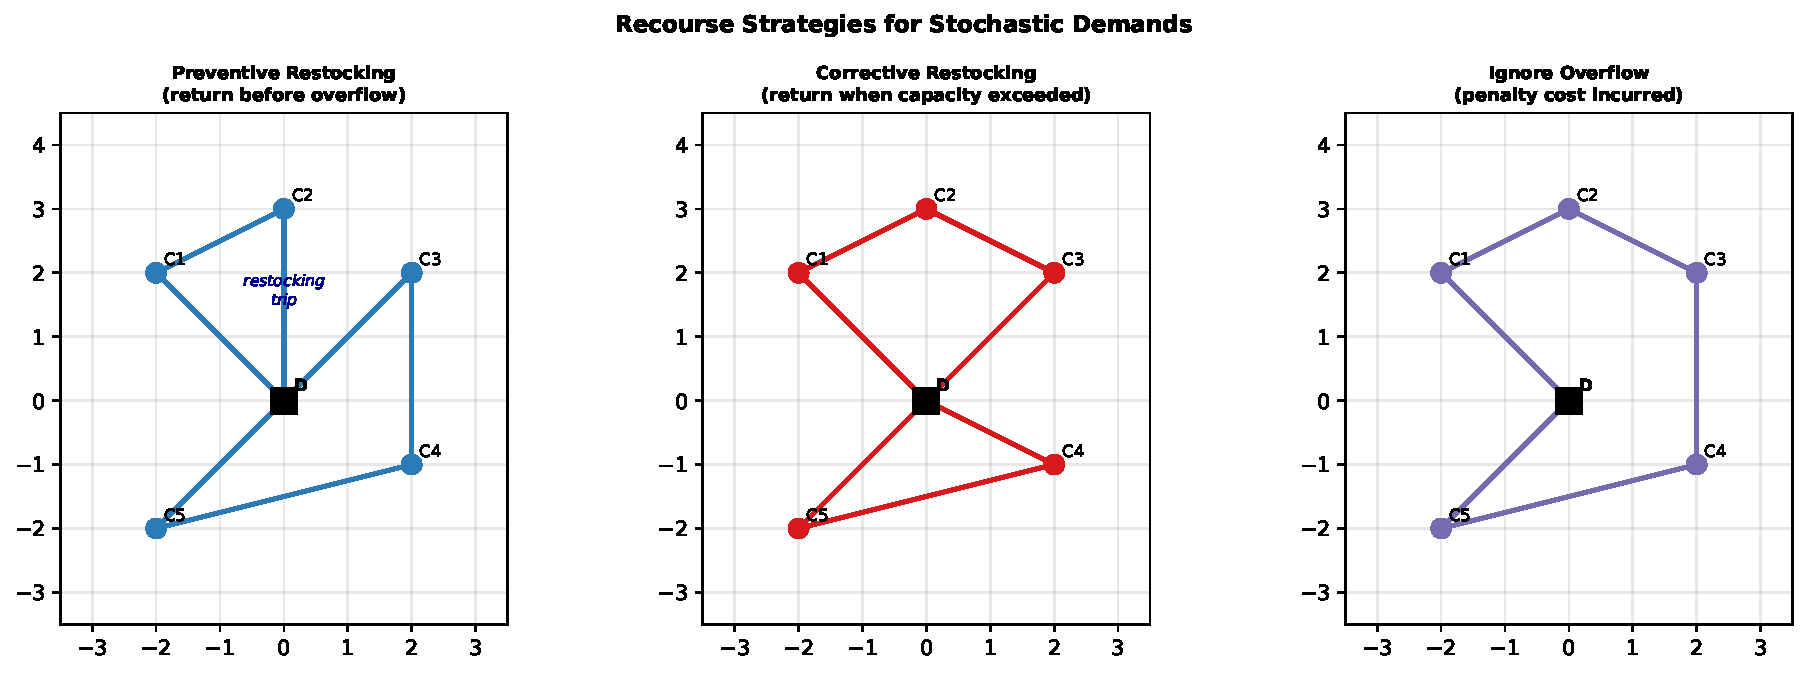
\includegraphics[width=0.80\textwidth]{fig_stochastic_demands_recourse.pdf}
    \caption{Three recourse strategies for stochastic demands.
             Left: preventive restocking (return to depot before capacity is
             exceeded, as a precaution).
             Centre: corrective restocking (return only when capacity is
             actually exceeded).
             Right: no restocking (incur a penalty cost for overflow).}
  \end{figure}

  \framebreak

  \begin{block}{Chance Constraints for VRPSD}
    An alternative to recourse is to impose a
    \textbf{chance constraint}: require that the probability of a
    capacity violation on each route is at most $\varepsilon$ (epsilon,
    a small number like 0.05):
    \[
      P\!\left(\sum_{i \in S_r} \xi_i > Q\right) \;\leq\; \varepsilon
      \quad \forall \text{ route } r
    \]
    Here $S_r$ is the set of customers on route~$r$, and $\varepsilon$ is
    the maximum allowed probability of route failure.

    This constraint says: ``the chance that the total demand on route~$r$
    exceeds the vehicle capacity must be no greater than $\varepsilon$''.
    The route is \emph{robust} if $\varepsilon$ is small (e.g.\ 5\%).
  \end{block}

  \begin{figure}
    \centering
    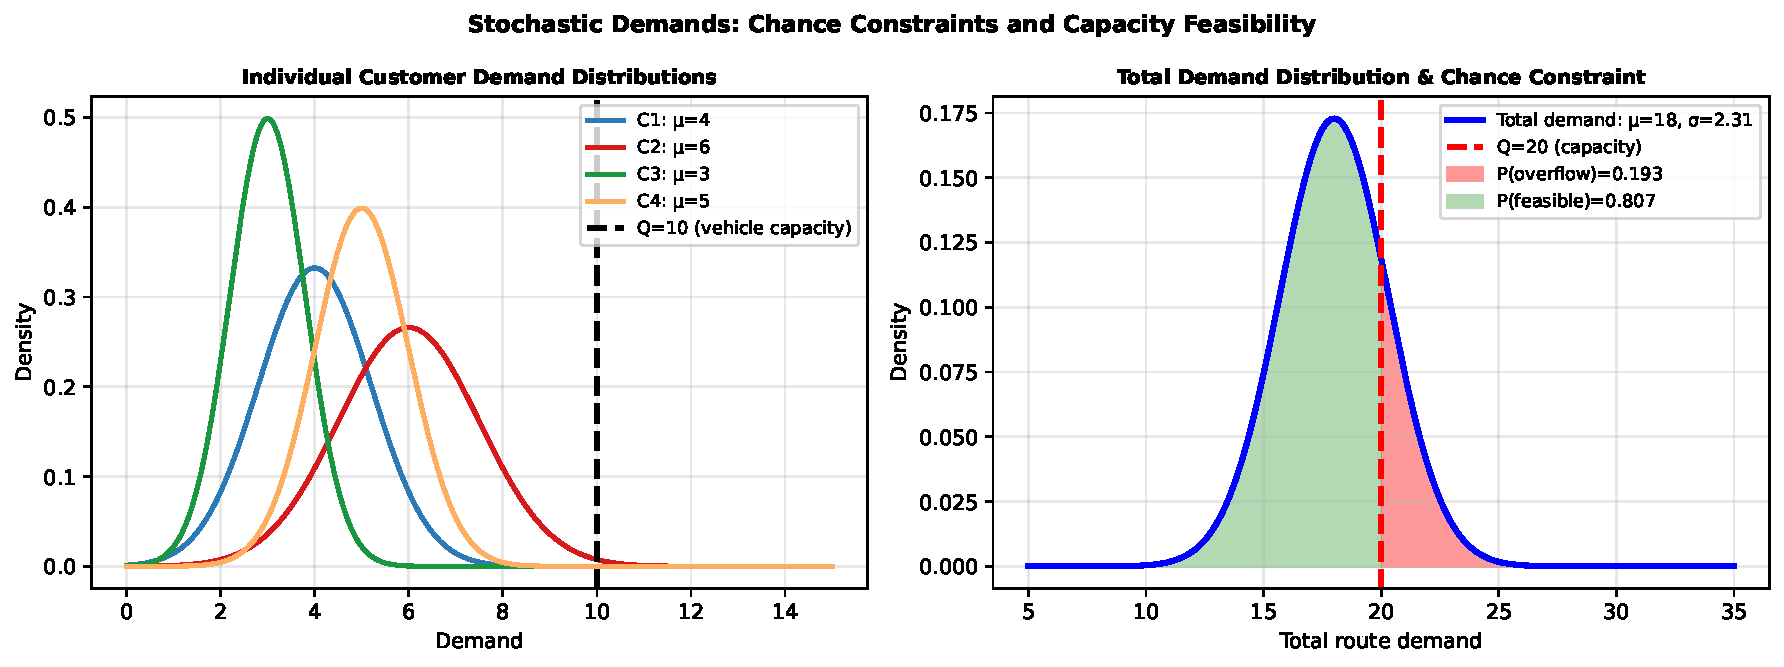
\includegraphics[width=0.72\textwidth]{fig_chance_constraint.pdf}
    \caption{Left: individual demand distributions for four customers.
             Right: the total route demand distribution and the chance
             constraint threshold (vehicle capacity~$Q$).  The red area
             is $P(\text{overflow})$; the green area is $P(\text{feasible})$.}
  \end{figure}

  \framebreak

  \begin{block}{Recourse Strategy Details: Preventive vs.\ Corrective}
    Let $L_k$ (L sub~$k$) denote the vehicle load after visiting the
    first $k$ customers in the planned order.

    \textbf{Preventive restocking}: the vehicle returns to the depot
    \emph{before} visiting customer~$k$ if the expected remaining demand
    from customer~$k$ onwards would cause overflow.
    Formally, return if $L_{k-1} + \mu_k > Q$.
    This is conservative but avoids route failure.

    \textbf{Corrective restocking}: the vehicle drives to customer~$k$
    and, if $L_{k-1} + \xi_k > Q$ (actual demand causes overflow), it
    returns to the depot to reload and then comes back to serve customer~$k$.
    This is the most common model in the literature, and is what we
    described in the network flow formulation above.

    \textbf{Emergency restocking}: allow partial delivery, deliver as
    much as the vehicle has left, and then return for the remainder.
    This adds additional route segments.
  \end{block}

  \framebreak

  The chapter discusses the following algorithmic approaches for VRPSD:

  \begin{enumerate}
    \item \textbf{Exact methods}: Integer L-shaped algorithm
          (Laporte, Louveaux, van Hamme, 1994) and branch-and-price
          (Gendreau, Laporte, Seguin, 1996).
          Can solve instances with up to 50 customers optimally.

    \item \textbf{Tabu search metaheuristic} (Gendreau, Laporte, Seguin,
          1996): a neighbourhood search where moves are ``banned'' (tabu)
          for a short time after being applied, to escape local optima.
          Produces solutions within 1--2\% of optimum for instances
          with up to 100 customers.

    \item \textbf{Simulated annealing}: accepts some worsening moves with
          a probability that decreases over time (the analogy is to slow
          cooling in metallurgy), allowing escape from local optima.

    \item \textbf{Genetic algorithms}: maintain a \emph{population} of
          candidate solutions and evolve them through crossover (combining
          parts of two solutions) and mutation (small random changes).
  \end{enumerate}

  \begin{alertblock}{Key Insight}
    Even for moderate-sized instances ($n \approx 50$), the exact expected
    recourse cost requires integrating over all demand scenarios, which is
    computationally expensive.
    The main contribution of the integer L-shaped algorithm is to avoid
    evaluating the full expected recourse cost at every iteration,
    instead using \emph{lower bounding cuts} that are much cheaper to compute.
  \end{alertblock}

\end{frame}

% ---------------------------------------------------------------------------
\begin{frame}[fragile]{Python: Simulating Expected Recourse Cost (VRPSD)}
\begin{lstlisting}
import numpy as np

def simulate_recourse_cost(route, demands_samples, depot_dists, Q):
    """
    Estimate E[Q(sigma, xi)] by Monte Carlo simulation.

    Parameters
    ----------
    route         : list of customer indices (0-indexed), e.g. [0,2,4,1,3]
    demands_samples : 2D array of shape (S, n), where S = number of scenarios
                    and n = number of customers.  demands_samples[s][i] is the
                    demand of customer i in scenario s.
    depot_dists   : 1D array of length n; depot_dists[i] = distance depot<->customer i
    Q             : vehicle capacity (maximum load)

    Returns
    -------
    expected_recourse : float, the estimated E[Q(sigma, xi)]
    """
    S = demands_samples.shape[0]
    total_recourse = 0.0

    for s in range(S):
        xi = demands_samples[s]   # demand vector for this scenario
        load = 0.0
        recourse_cost = 0.0
        for cust in route:
            if load + xi[cust] > Q:
                # Capacity exceeded: return to depot and reload
                recourse_cost += 2 * depot_dists[cust]
                load = 0.0      # vehicle reloaded at depot
            load += xi[cust]    # serve this customer
        total_recourse += recourse_cost

    return total_recourse / S   # average over all scenarios


# Example: 4 customers, Q=10, 5000 Monte Carlo scenarios
np.random.seed(42)
n_customers = 4
S_scenarios = 5000
Q_cap = 10
# Each customer demand ~ Normal(mean, std), clipped at 0
means   = [3.0, 4.0, 2.5, 3.5]
stds    = [0.8, 1.2, 0.6, 1.0]
samples = np.column_stack([
    np.maximum(0, np.random.normal(mu, sig, S_scenarios))
    for mu, sig in zip(means, stds)
])
depot_d = [2.1, 3.5, 1.8, 2.9]   # distances from depot to each customer

route_A = [0, 1, 2, 3]  # visit customers in order 1,2,3,4
route_B = [2, 0, 3, 1]  # a different ordering

cost_A = simulate_recourse_cost(route_A, samples, depot_d, Q_cap)
cost_B = simulate_recourse_cost(route_B, samples, depot_d, Q_cap)
print(f"Expected recourse cost, route A: {cost_A:.3f}")
print(f"Expected recourse cost, route B: {cost_B:.3f}")
# Route with smaller expected recourse cost is preferred.
\end{lstlisting}
\end{frame}

% ===========================================================================
\section{Stochastic Customers}
% ===========================================================================

\begin{frame}[allowframebreaks]{Stochastic Customers: The VRPSC}

  The \textbf{Vehicle Routing Problem with Stochastic Customers (VRPSC)}
  considers the case where it is uncertain which customers will actually
  need service.
  Each customer~$i$ is present (has a demand) independently with
  probability $p_i$ (p sub~$i$), and absent with probability $1-p_i$.

  \begin{block}{Difference from VRPSD}
    In the VRPSD, every customer is definitely present but has an unknown
    demand.  In the VRPSC, the demand per customer is fixed (say, one unit),
    but the set of customers to serve is random.
    Customers who are absent when the vehicle arrives are simply skipped,
    and the vehicle continues to the next customer in its planned tour.
  \end{block}

  This problem was first studied in the context of the
  \textbf{Probabilistic Travelling Salesman Problem (PTSP)},
  introduced by Jaillet (1985) and Bertsimas (1988).
  The PTSP is the single-vehicle version.

  \begin{figure}
    \centering
    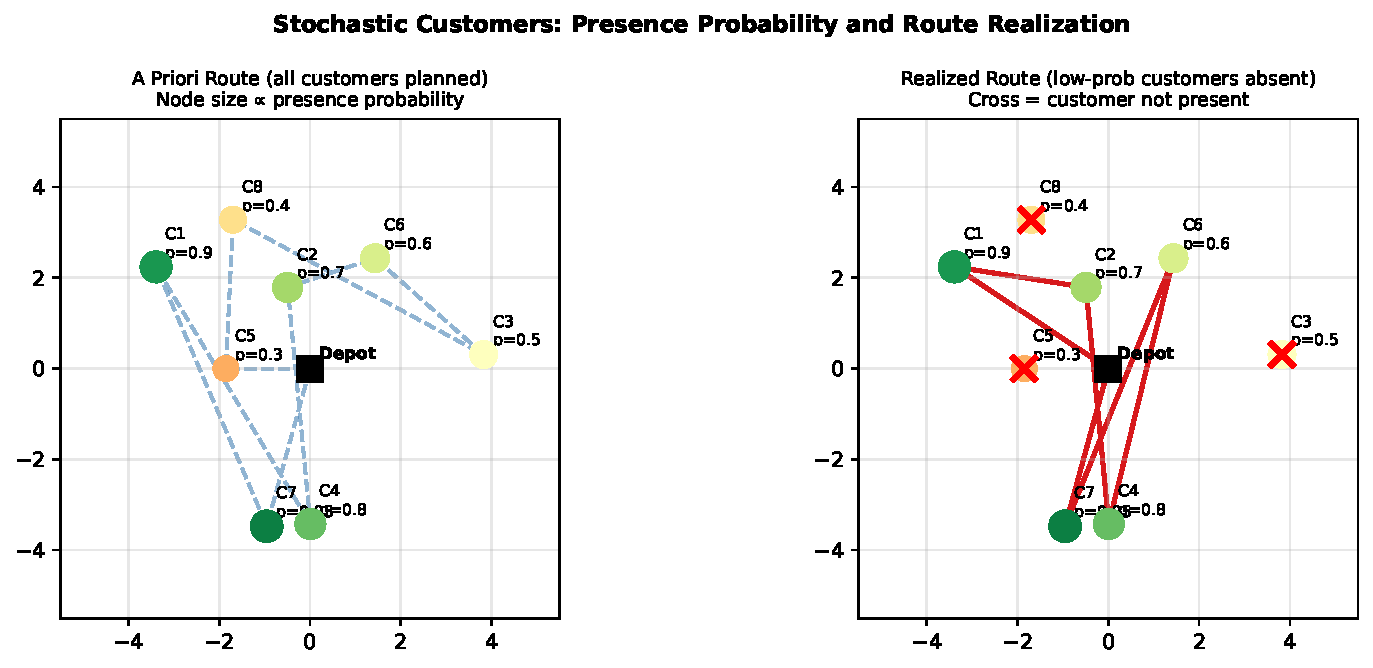
\includegraphics[width=0.75\textwidth]{fig_stochastic_customers.pdf}
    \caption{Left: the a~priori tour including all customers, with node
             size proportional to presence probability.
             Right: one realization where low-probability customers are
             absent (marked with red cross); the vehicle skips them
             following the a~priori order.}
  \end{figure}

  \framebreak

  \begin{block}{The Single-Location Model (VRPSC with One Vehicle)}
    Consider a single vehicle based at a depot~0.
    Customers are located at positions $v_1, \ldots, v_n$, each present
    independently with probability $p_i$.
    Let $\sigma = (\sigma_1, \sigma_2, \ldots, \sigma_n)$ be the a~priori
    tour.

    Given that customer $\sigma_k$ is present, the vehicle visits it;
    otherwise it drives directly to the next present customer in the sequence.
    The expected cost of the a~priori tour is:
    \begin{align*}
      \mathbb{E}[C(\sigma)] &= \sum_{i=1}^{n} \sum_{j > i}
      p_{\sigma_i} p_{\sigma_j}
      \prod_{k=i+1}^{j-1}(1-p_{\sigma_k})
      \cdot d(\sigma_i, \sigma_j)
    \end{align*}
    This sum accounts for all pairs $(\sigma_i, \sigma_j)$ of present
    customers where $\sigma_j$ is the successor of $\sigma_i$ in the
    realized tour (i.e., all customers between them in the a~priori order
    are absent).
    The product $\prod_{k=i+1}^{j-1}(1-p_{\sigma_k})$ is the probability
    that all intermediate customers are absent.
  \end{block}

  \framebreak

  \begin{figure}
    \centering
    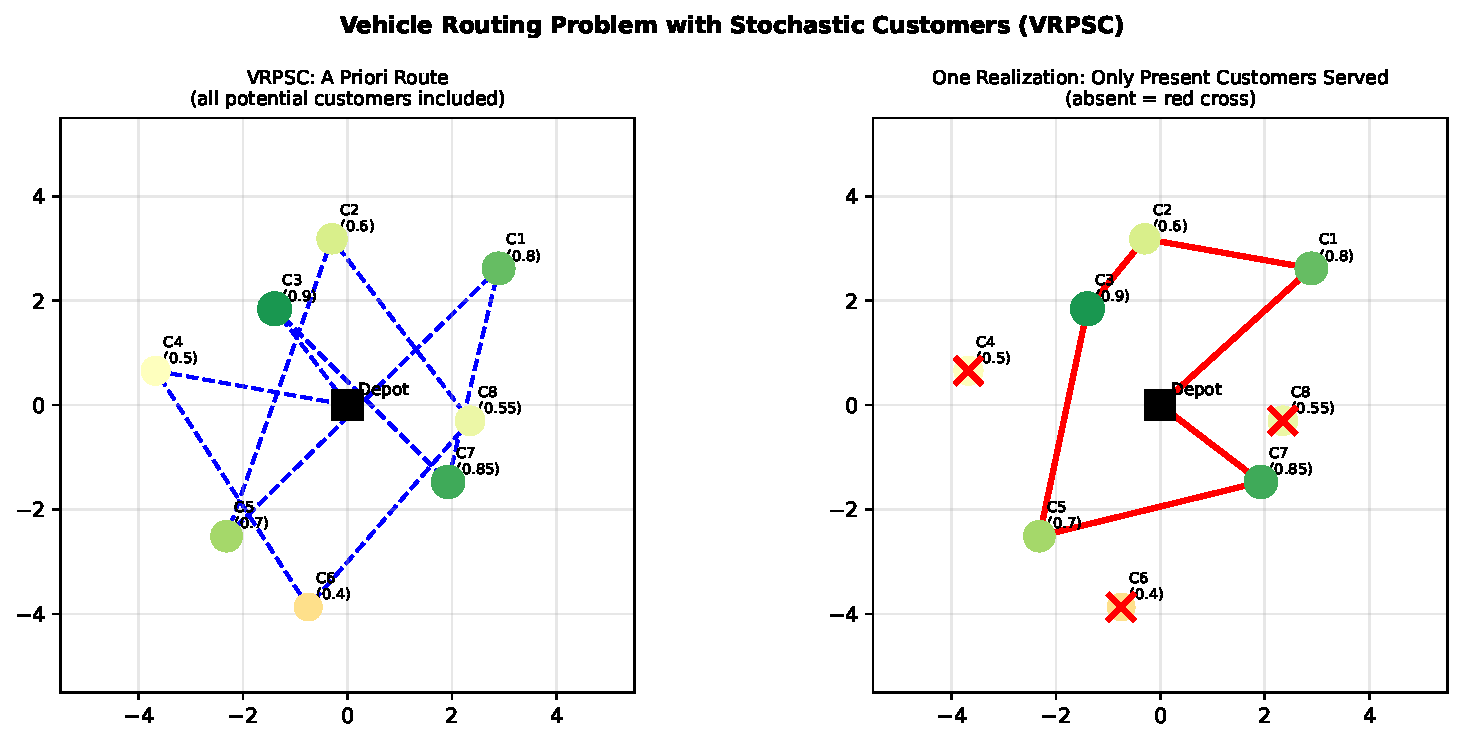
\includegraphics[width=0.72\textwidth]{fig_vrpsc_single_vehicle.pdf}
    \caption{VRPSC single-vehicle illustration.
             Left: the a~priori tour (planned for all customers).
             Right: one realization (only high-probability customers are
             present; low-probability customers are skipped).}
  \end{figure}

  \begin{exampleblock}{Worked Example: Expected VRPSC Cost with 3 Customers}
    Suppose the depot is at position~0, and there are 3 customers with
    positions $A, B, C$ at unit distances:
    $d(0,A)=1, d(A,B)=1, d(B,C)=1, d(C,0)=1, d(0,B)=\sqrt{2}, \ldots$

    Say the a~priori tour is $0 \to A \to B \to C \to 0$ and
    $p_A=0.9, p_B=0.6, p_C=0.8$.

    With probability $p_A \cdot p_B \cdot p_C = 0.9 \times 0.6 \times 0.8 = 0.432$,
    all three are present and the tour is $0\to A\to B\to C\to 0$.

    With probability $p_A \cdot (1-p_B) \cdot p_C = 0.9 \times 0.4 \times 0.8 = 0.288$,
    $B$ is absent: tour becomes $0\to A\to C\to 0$ (saving the $A\to B$
    and $B\to C$ edges, but paying $d(A,C)$ instead).

    Summing over all $2^3=8$ realizations gives the expected tour cost.
    Optimizing over all $n! / 2$ possible a~priori tours yields the
    optimal VRPSC solution.
  \end{exampleblock}

  \framebreak

  \begin{block}{Solution Approaches for VRPSC / PTSP}
    \begin{enumerate}
      \item \textbf{Exact branch-and-bound}: for small $n$ (up to~15).
            The expected cost of each tour is computed explicitly by
            summing over all $2^n$ realizations.

      \item \textbf{Savings-based heuristic}: apply the Clarke-Wright
            savings algorithm but using \emph{expected savings}
            $\mathbb{E}[s_{ij}]$ rather than deterministic savings.
            An expected saving $\mathbb{E}[s_{ij}]$ accounts for the
            probability that both customers $i$ and $j$ are present.

      \item \textbf{Tabu search on a~priori tours}: neighbourhood
            moves (2-opt, 3-opt, or-opt) are applied to permutations,
            with the expected cost evaluated at each step.

      \item \textbf{Genetic algorithm}: maintain a population of
            permutations; crossover and mutation operators are designed
            to preserve good sub-sequences.
    \end{enumerate}
  \end{block}

  The chapter reports that tabu search algorithms for the VRPSC can find
  solutions within 1\% of optimal for instances with up to 100 customers.

  \begin{alertblock}{Key Insight: Order Matters}
    Even though absent customers are simply skipped, the \emph{order}
    in which customers appear in the a~priori tour affects the expected
    cost.  Placing two customers with low presence probabilities next to
    each other is risky: if both are absent, the vehicle makes a long
    jump.  The optimal a~priori tour tends to interleave high- and
    low-probability customers.
  \end{alertblock}

\end{frame}

% ---------------------------------------------------------------------------
\begin{frame}[fragile]{Python: Expected Tour Cost for VRPSC}
\begin{lstlisting}
import numpy as np
from itertools import permutations

def expected_ptsp_cost(tour, probs, dist_matrix):
    """
    Compute the exact expected tour cost for the PTSP (single-vehicle VRPSC).

    Parameters
    ----------
    tour        : list, e.g. [0, 1, 2, 3] (0 = depot; others are customers)
    probs       : dict {customer_id: presence_probability}
                  e.g. {1: 0.9, 2: 0.6, 3: 0.8}
    dist_matrix : 2D array; dist_matrix[i][j] = distance from i to j

    Returns
    -------
    E_cost : float, expected total tour distance
    """
    customers = [t for t in tour if t != 0]   # exclude depot
    n = len(customers)
    E_cost = 0.0

    # Enumerate all 2^n subsets of customers that could be present
    for mask in range(1 << n):
        prob_scenario = 1.0
        present = [0]  # depot always included
        for k, c in enumerate(customers):
            if mask & (1 << k):
                present.append(c)
                prob_scenario *= probs[c]
            else:
                prob_scenario *= (1 - probs[c])

        present.append(0)   # return to depot

        # Compute route cost for this realization following the a priori order
        route_cost = 0.0
        for idx in range(len(present)-1):
            route_cost += dist_matrix[present[idx]][present[idx+1]]

        E_cost += prob_scenario * route_cost

    return E_cost


# Demonstration: 3 customers, find the best a priori tour
n_cust = 3
# Distance matrix (depot=0, customers=1,2,3)
D = np.array([
    [0,  2.0, 3.0, 2.5],
    [2.0, 0,  1.5, 2.0],
    [3.0, 1.5, 0,  1.0],
    [2.5, 2.0, 1.0, 0 ],
])
p = {1: 0.9, 2: 0.6, 3: 0.8}

best_cost = float('inf')
best_tour = None
for perm in permutations([1, 2, 3]):
    tour = [0] + list(perm) + [0]
    ec = expected_ptsp_cost(tour, p, D)
    if ec < best_cost:
        best_cost, best_tour = ec, tour

print(f"Optimal a priori tour: {best_tour}")
print(f"Expected cost: {best_cost:.4f}")
\end{lstlisting}
\end{frame}

% ===========================================================================
\section{Stochastic Travel Times}
% ===========================================================================

\begin{frame}[allowframebreaks]{Stochastic Travel Times: Time-Window Feasibility}

  The \textbf{VRP with Stochastic Travel Times (VRPST)} (also called the
  VRP with stochastic service times) addresses the situation where the time
  to travel between two locations is uncertain, typically due to variable
  traffic conditions.

  \begin{block}{What Makes This Different?}
    In the VRPSD and VRPSC, stochasticity affects \emph{load feasibility}
    (whether the vehicle can carry all demanded goods).
    In the VRPST, stochasticity affects \emph{time feasibility}: a customer
    may have a time window $[a_i, b_i]$ (earliest and latest arrival time),
    and the vehicle may arrive too early (must wait, incurring a waiting
    cost) or too late (violates the time window, incurring a penalty).
  \end{block}

  \begin{block}{Two Components of Stochastic Service Time}
    The total time to serve customer~$i$ after departing from customer~$j$
    has two random components:
    \begin{enumerate}
      \item \textbf{Travel time} $t_{ij}$ (t sub $i$-$j$): random, affected
            by traffic, weather, road conditions.
      \item \textbf{Service time} $s_i$ (s sub~$i$): random, affected by
            how long the unloading takes, customer's readiness, etc.
    \end{enumerate}
    The sum $T_{ij} = t_{ij} + s_i$ is the total stochastic time from
    departing~$j$ to completing service at~$i$.
  \end{block}

  \framebreak

  \begin{figure}
    \centering
    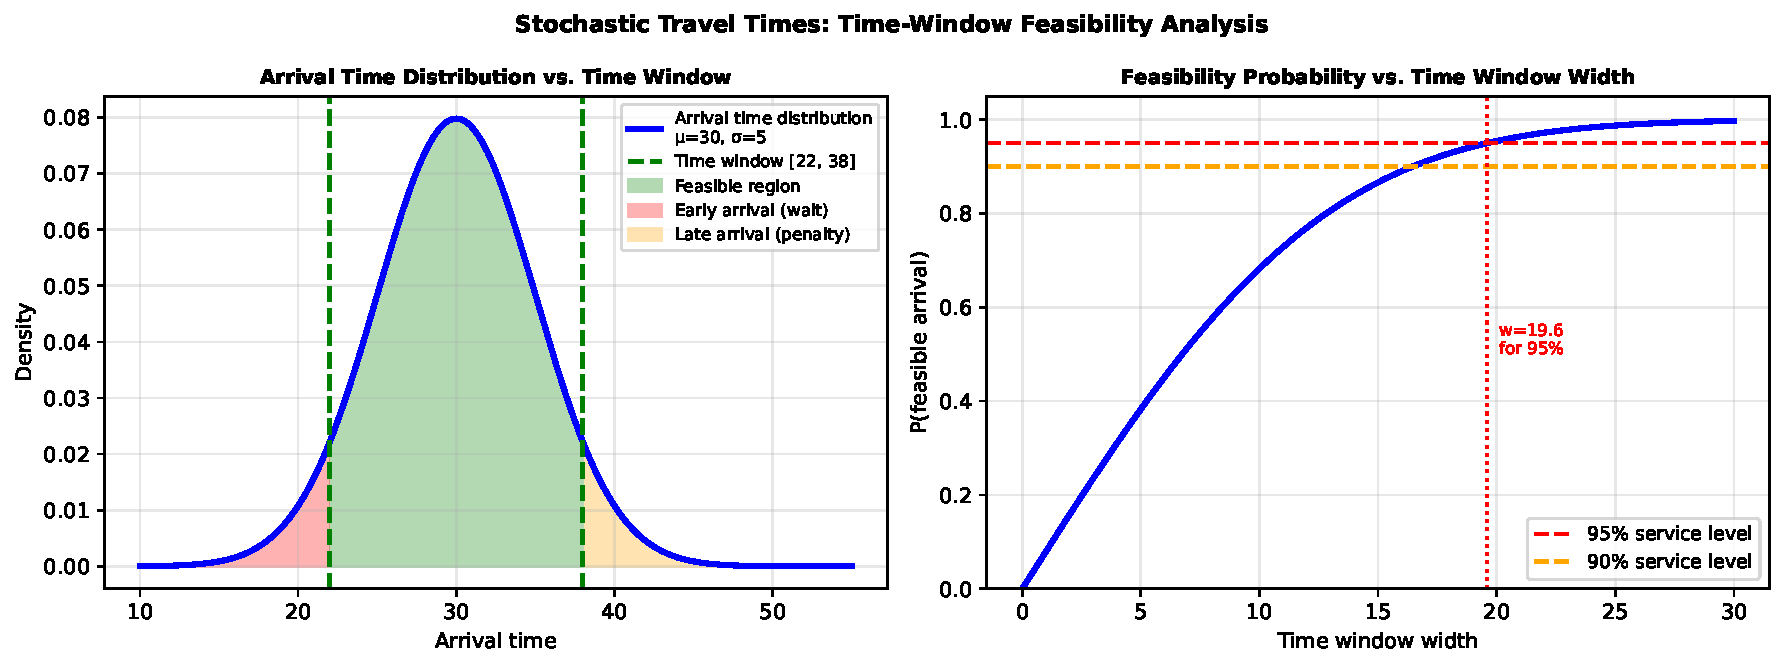
\includegraphics[width=0.80\textwidth]{fig_stochastic_travel_times.pdf}
    \caption{Left: the arrival time distribution (bell curve) at a customer
             relative to the time window $[a, b]$.
             Green area = on-time probability.
             Red area = early arrival (vehicle must wait).
             Orange area = late arrival (time-window violation, penalty).
             Right: the probability of feasible arrival increases as the
             time window width grows.}
  \end{figure}

  \framebreak

  \begin{block}{Objective Function with Expected Penalties}
    The VRPST objective minimizes expected total route cost including
    waiting and late-arrival penalties:
    \[
      \min_{\mathbf{x}} \;\; \sum_{(i,j)} c_{ij} x_{ij}
      \;+\; \alpha \sum_i \mathbb{E}[\max(0,\, a_i - A_i)]
      \;+\; \beta  \sum_i \mathbb{E}[\max(0,\, A_i - b_i)]
    \]
    where:
    \begin{itemize}
      \item $A_i$ (A sub~$i$) --- the \emph{random arrival time} at
            customer~$i$ (it is random because travel times are random).
      \item $a_i$ (a sub~$i$) --- the \emph{earliest} acceptable arrival
            time at customer~$i$ (left bound of time window).
      \item $b_i$ (b sub~$i$) --- the \emph{latest} acceptable arrival
            time at customer~$i$ (right bound of time window).
      \item $\alpha$ (alpha) --- the penalty per unit time of early
            arrival (waiting cost per unit time).
      \item $\beta$ (beta) --- the penalty per unit time of late arrival
            (larger than $\alpha$ in practice: missing a time window is
            more costly than waiting).
      \item $\max(0, a_i - A_i)$ --- the positive waiting time
            (zero if arrival is not early).
      \item $\max(0, A_i - b_i)$ --- the positive lateness
            (zero if arrival is within the time window).
    \end{itemize}
  \end{block}

  \framebreak

  \begin{alertblock}{How to Read the VRPST Objective}
    This objective function says: ``choose routes that minimize the total
    travel cost plus the average cost of being too early (waiting at a
    customer) plus the average cost of being too late (violating the time
    window).''
    As $\alpha \to 0$ (no waiting cost), the model encourages departing
    very early to avoid lateness.
    As $\beta \to 0$ (no penalty for lateness), the model ignores time
    windows entirely.
    Balancing $\alpha$ and $\beta$ captures the real-world trade-off
    between being punctual and minimizing travel time.
  \end{alertblock}

  \begin{block}{Robust Scheduling Approach}
    Rather than minimizing expected penalties, the \emph{robust
    scheduling} approach requires that every time window is met with at
    least probability $1-\varepsilon$ (chance constraint on time feasibility):
    \[
      P(a_i \leq A_i \leq b_i) \;\geq\; 1-\varepsilon
      \quad \forall i
    \]
    If travel times are normally distributed with mean $\mu_{ij}$ and
    variance $\sigma_{ij}^2$ (sigma sub $i$-$j$ squared), this chance
    constraint translates to a \emph{deterministic constraint} on the
    departure time using the inverse normal CDF (the z-score).
  \end{block}

  \framebreak

  \begin{block}{Algorithms for VRPST}
    The VRPST has been studied primarily with heuristic approaches, since
    the expected penalties involve integration over the joint distribution
    of arrival times at \emph{all} customers simultaneously (which
    correlates through the sequence of travel times):

    \begin{enumerate}
      \item \textbf{Monte Carlo simulation + local search}: evaluate
            candidate routes by simulating many travel-time scenarios
            and averaging the total cost.  Apply 2-opt and or-opt
            neighbourhood moves.

      \item \textbf{Stochastic programming with scenario trees}:
            discretize the travel-time distribution into $S$ scenarios
            and solve the resulting deterministic large-scale LP/MIP.

      \item \textbf{Robust optimization}: choose routes that perform
            well in the \emph{worst-case} travel-time scenario within
            an uncertainty set (e.g., all travel times within
            $\pm 2\sigma_{ij}$ of their means).
    \end{enumerate}
  \end{block}

  The key observation from the computational results in the chapter is
  that \emph{time-window feasibility under stochastic travel times is
  highly sensitive to the variance of the travel times}: even modest
  variance can make a seemingly tight time-window plan infeasible with
  significant probability, and robust routes tend to include more
  buffer time but at higher route cost.

\end{frame}

% ===========================================================================
\section{Conclusions and Future Research Directions}
% ===========================================================================

\begin{frame}[allowframebreaks]{Conclusions}

  This chapter has surveyed the three main classes of Stochastic Vehicle
  Routing Problems and the principal solution methods for each.

  \begin{block}{What We Have Covered}
    \begin{enumerate}
      \item \textbf{A priori optimization}: build a complete route plan
            before uncertainty is resolved, evaluate it by its expected
            cost under a fixed recourse policy (re-supply when capacity
            is exceeded).  Key algorithms: integer L-shaped method,
            branch-and-price.

      \item \textbf{Reoptimization model}: adapt the route plan online as
            information is revealed.  Formulated as a Markov Decision
            Process; solved approximately by rollout heuristics and
            re-solve policies.

      \item \textbf{Probabilistic (expected-cost) formulation}: minimize
            the true expected total cost over all random scenarios;
            approximated by Sample Average Approximation.

      \item \textbf{Stochastic demands (VRPSD)}: uncertainty in customer
            demands; handle by chance constraints or recourse (preventive
            or corrective restocking).

      \item \textbf{Stochastic customers (VRPSC/PTSP)}: uncertainty in
            which customers are present; optimize a~priori tour order to
            minimize expected distance when absent customers are skipped.

      \item \textbf{Stochastic travel times (VRPST)}: uncertainty in
            travel and service times; time-window feasibility becomes
            probabilistic; objective includes expected waiting and
            late-arrival penalties.
    \end{enumerate}
  \end{block}

  \framebreak

  \begin{figure}
    \centering
    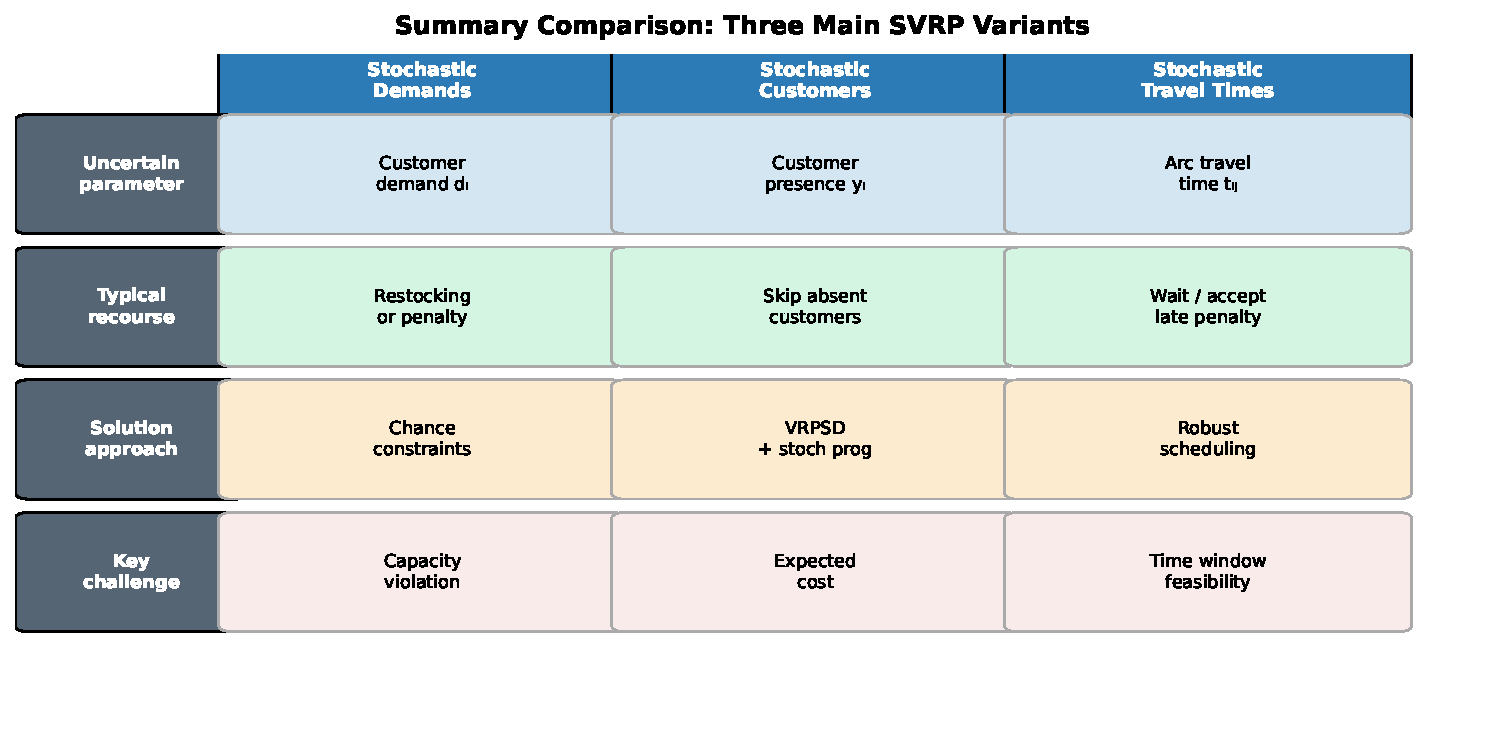
\includegraphics[width=0.78\textwidth]{fig_svrp_summary.pdf}
    \caption{Summary comparison of the three main SVRP variants:
             uncertain parameter, typical recourse action, solution
             approach, and key challenge.}
  \end{figure}

  \framebreak

  \begin{block}{Future Research Directions}
    The chapter identifies the following open problems and research
    directions as of the time of writing (2014):

    \begin{enumerate}
      \item \textbf{Multi-period and multi-echelon SVRP}: combining
            stochasticity with multiple depots, multiple time periods,
            or multi-level supply chains.

      \item \textbf{Integration with inventory management}: joint
            optimization of routing and replenishment decisions when
            customer demand is stochastic over time.

      \item \textbf{Richer uncertainty models}: correlated demands
            (e.g., seasonal effects causing nearby customers' demands
            to be positively correlated), non-stationary distributions,
            and demand learning over time.

      \item \textbf{Robust and distributionally robust formulations}:
            optimizing for the worst-case distribution within a class
            (e.g., all distributions with given mean and variance),
            protecting against model misspecification.

      \item \textbf{Large-scale heuristics}: most current exact methods
            are limited to $n \leq 50$.  Developing effective
            metaheuristics and approximation algorithms for $n \geq 200$
            is an important practical goal.

      \item \textbf{Dynamic VRP}: combining stochastic modelling with
            real-time information updates from GPS, traffic monitoring,
            and demand signals.

      \item \textbf{Machine learning integration}: using historical data
            to learn demand distributions, predict customer presence,
            and warm-start optimization algorithms.
    \end{enumerate}
  \end{block}

  \framebreak

  \begin{alertblock}{The Central Lesson of Stochastic VRP}
    In any real-world routing application, ignoring uncertainty leads to
    plans that look optimal on paper but perform poorly in practice.
    The stochastic VRP framework provides principled tools to incorporate
    uncertainty: by modelling random parameters explicitly, optimizing
    expected costs, and designing policies that adapt gracefully when
    reality deviates from expectation.
    The computational cost of these methods is higher than for
    deterministic VRP, but the benefit---more reliable, cheaper-in-practice
    routes---is usually worth it.
  \end{alertblock}

\end{frame}

% ===========================================================================
\section{Bibliography}
% ===========================================================================

\begin{frame}[allowframebreaks]{Selected Bibliography}

  The following works are cited in this chapter.
  References are grouped by topic for easier navigation.

  \textbf{A Priori Optimization and Integer L-Shaped Method:}
  \begin{itemize}
    \item Laporte, G., Louveaux, F.V., and van Hamme, L. (1994).
          An integer L-shaped algorithm for the capacitated vehicle routing
          problem with stochastic demands.
          \emph{Operations Research}, 10(1), 10--23.
    \item Gendreau, M., Laporte, G., and Seguin, R. (1996).
          Stochastic vehicle routing.
          \emph{European Journal of Operational Research}, 88(1), 3--12.
    \item Christiansen, C.H. and Lysgaard, J. (2007).
          A branch-and-price algorithm for the capacitated vehicle routing
          problem with stochastic demands.
          \emph{Operations Research Letters}, 35(6), 773--781.
  \end{itemize}

  \textbf{Probabilistic TSP and Stochastic Customers:}
  \begin{itemize}
    \item Jaillet, P. (1988).
          A priori solution of a travelling salesman problem in which
          a random subset of the customers are visited.
          \emph{Operations Research}, 36(6), 929--936.
    \item Bertsimas, D.J., Jaillet, P., and Odoni, A. (1990).
          A priori optimization.
          \emph{Operations Research}, 38(6), 1019--1033.
    \item Laporte, G., Louveaux, F.V., and Mercure, H. (1989).
          Models and exact solutions for a class of stochastic location-routing
          problems.
          \emph{European Journal of Operational Research}, 39(1), 71--78.
  \end{itemize}

  \framebreak

  \textbf{Stochastic Travel Times:}
  \begin{itemize}
    \item Laporte, G., Louveaux, F.V., and Mercure, H. (1992).
          The vehicle routing problem with stochastic travel times.
          \emph{Transportation Science}, 26(3), 161--170.
    \item Kenyon, A.S. and Morton, D.P. (2003).
          Stochastic vehicle routing with random travel times.
          \emph{Transportation Science}, 37(1), 69--82.
  \end{itemize}

  \textbf{Metaheuristics for SVRP:}
  \begin{itemize}
    \item Gendreau, M., Laporte, G., and Seguin, R. (1996).
          A tabu search heuristic for the vehicle routing problem with
          stochastic demands and customers.
          \emph{Operations Research}, 44(3), 469--477.
    \item Secomandi, N. (2000).
          Comparing neuro-dynamic programming algorithms for the vehicle
          routing problem with stochastic demands.
          \emph{Computers \& Operations Research}, 27(11--12), 1201--1225.
    \item Hvattum, L.M., Lokketangen, A., and Laporte, G. (2006).
          Solving a dynamic and stochastic vehicle routing problem with
          a sample scenario hedging heuristic.
          \emph{Transportation Science}, 40(4), 421--438.
  \end{itemize}

  \textbf{Books and Surveys:}
  \begin{itemize}
    \item Birge, J.R. and Louveaux, F. (2011).
          \emph{Introduction to Stochastic Programming}, 2nd ed.
          Springer.
    \item Powell, W.B., Jaillet, P., and Odoni, A. (1995).
          Stochastic and dynamic networks and routing.
          In: Ball et al.\ (eds.), \emph{Handbooks in Operations Research
          and Management Science: Network Routing}.
  \end{itemize}

\end{frame}

% ─────────────────────────────────────────────────────────────────────────────
\end{document}
